
\chapter{On the Transferability of Lottery Winners} % Chapter title
\label{ch:tl_lth} % For referencing the chapter elsewhere, use \autoref{ch:introduction} 

\begin{remark}{Contributions and Outline}
	In Chapters \ref{ch:tl_natural_to_non_natural} and \ref{ch:minerva}, we have always performed Transfer Learning (TL) with large and deep convolutional neural networks, as this is the type of models which have obtained state-of-the-art results in the naturalistic domain. While all the studies presented so far aimed at characterizing the TL properties of popular convolutional architectures, we explore a different approach in this chapter. We use TL as a tool for not only exploiting the performance of pre-trained neural networks but also for characterizing a relatively new deep learning phenomenon that comes with the name of the ``Lottery Ticket Hypothesis" (LTH). Specifically, we investigate whether lottery winners found on datasets of natural images contain inductive biases that are generic enough to generalize to non-natural image distributions. To do so, we present the first results that study the transferability of winning initializations in this particular training setting. Furthermore, we also show that the LTH offers a novel way for doing TL when the training data is scarce. The rest of this chapter is structured as follows: Sec. \ref{sec:intro} introduces the LTH and presents the reasons that have motivated studying this phenomenon from a TL perspective. Sec. \ref{sec:datasets} and Sec. \ref{sec:experimental_setup} present the experimental setup that was used throughout this chapter, while Sec. \ref{sec:results} and Sec. \ref{sec:additional_studies} present the main findings of our research. The chapter ends by contextualizing its content with respect to the existing literature in Sec. \ref{sec:related_work} and by identifying some potential avenues for future work in Sec. \ref{sec:conclusion}.

\vspace{5mm}
\textit{This chapter is based on the publication \citet{sabatelli2020transferability}.}

\end{remark}

\section{The Lottery Ticket Hypothesis}
\label{sec:intro}
The \textcolor{RoyalBlue}{``Lottery-Ticket-Hypothesis"} (LTH) \cite{frankle2018lottery} states that within large randomly initialized neural networks, there exist smaller sub-networks which, if trained from their initial weights, can perform just as well as the fully trained unpruned network from which they are extracted. This happens to be possible because the weights of these sub-networks seem to be particularly well initialized before training starts, therefore making these smaller architectures suitable for learning (see Fig \ref{fig:tickets_visualization} for an illustration). These sub-networks, i.e., the pruned structure and their initial weights, are called winning tickets, as they appear to have won the initialization lottery. Since winning tickets only contain a very limited amount of parameters, they yield faster training, inference, and sometimes even better final performance than their larger over-parametrized counterparts \cite{frankle2018lottery,franklestabilizing}. So far, winning tickets are typically identified by an iterative procedure that cycles through several steps of network training and weight pruning, starting from a randomly initialized unpruned network. While simple and intuitive, the resulting algorithm has, unfortunately, a high computational cost. Even though the resulting sparse networks can be trained efficiently and in isolation from their initial weights, the LTH idea has not yet led to more efficient solutions for training a sparse network than existing pruning algorithms that all also require to first fully train an unpruned network \cite{han2015deep,molchanov2016pruning,dong2017learning,lin2017runtime,zhuang2018discrimination}.

\begin{figure*}[!htb]
\minipage{0.3\textwidth}
  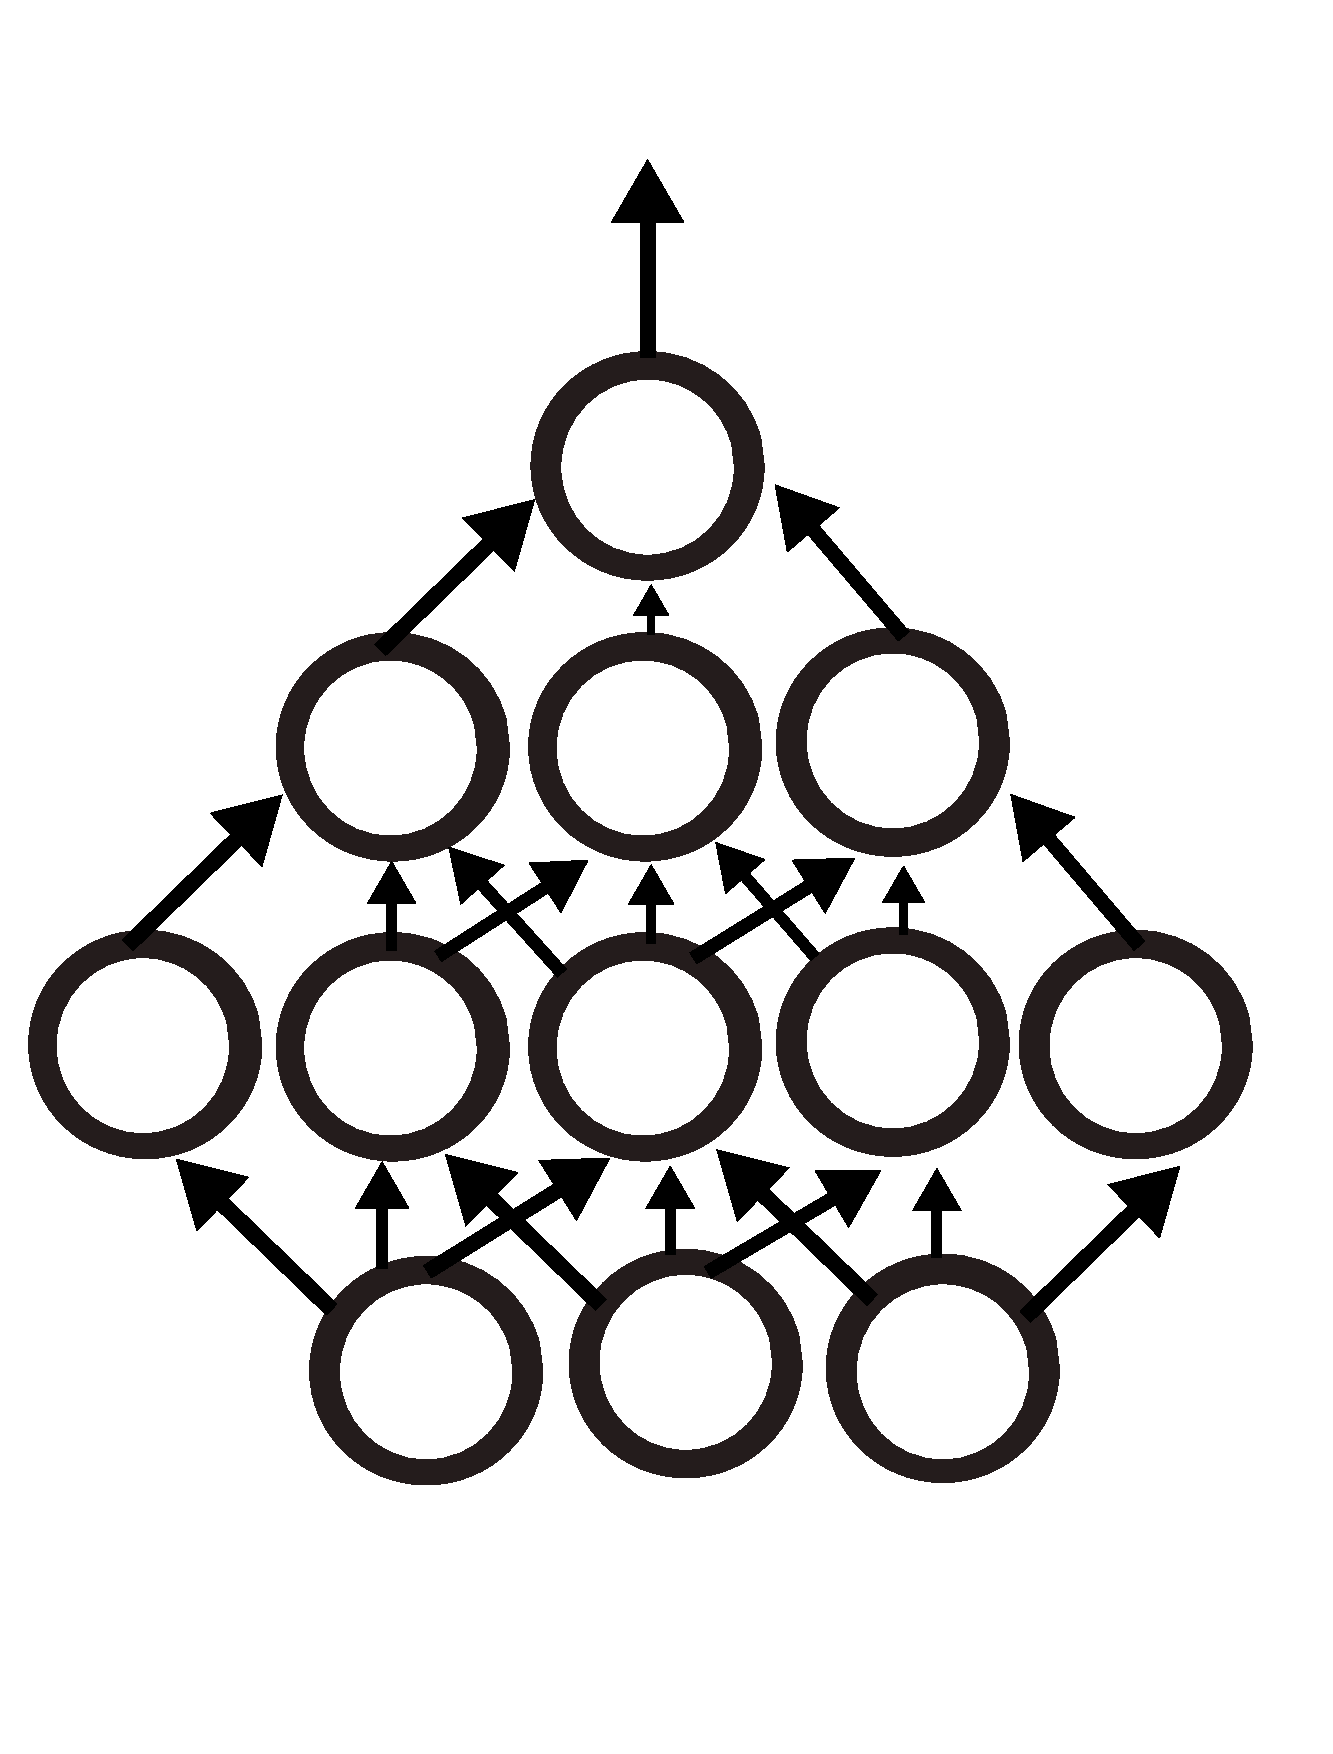
\includegraphics[width=\linewidth]{./Images/Chapter06/mlp.pdf}
\endminipage\hfill
\minipage{0.3\textwidth}
  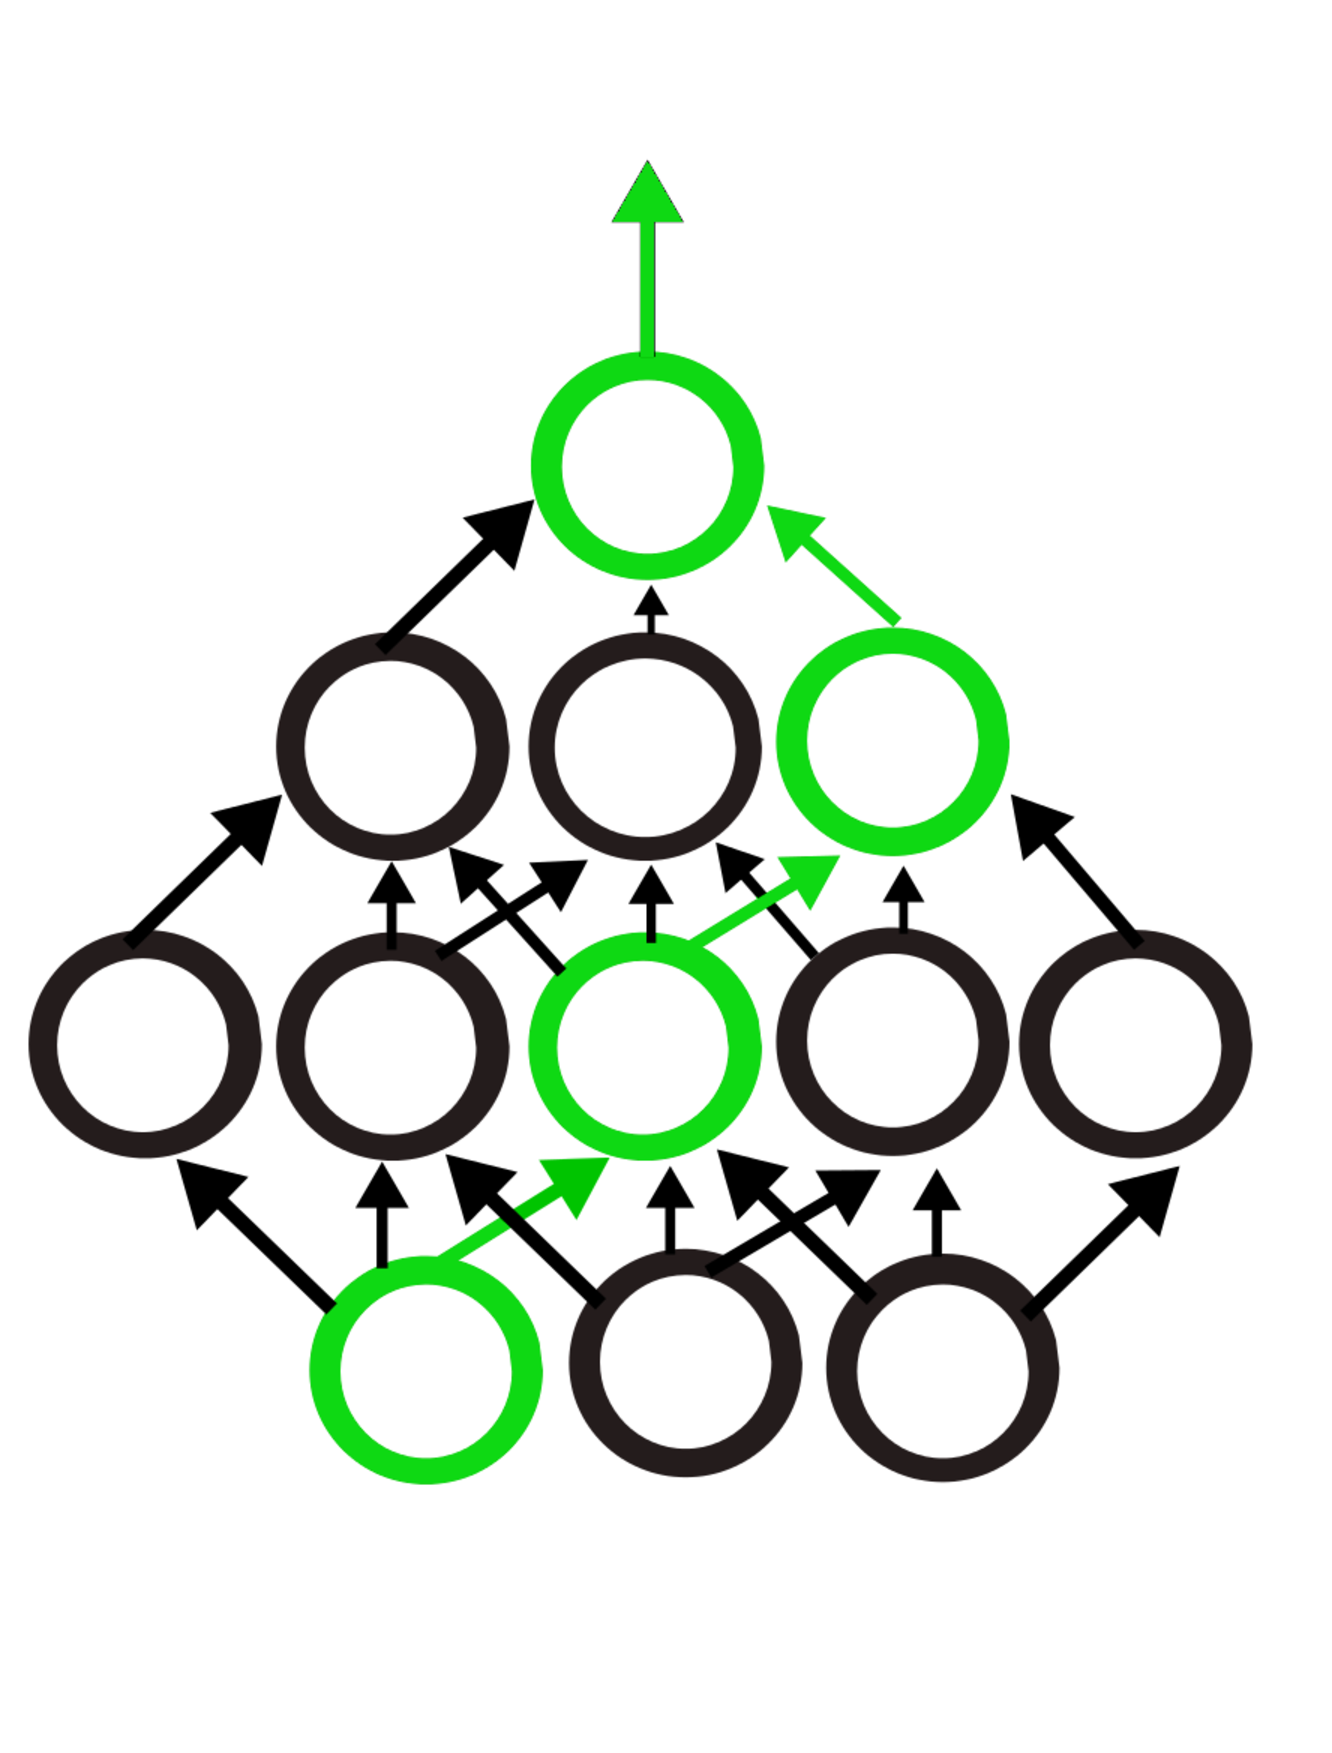
\includegraphics[width=\linewidth]{./Images/Chapter06/mlp_ticket_3.pdf}
\endminipage\hfill
\minipage{0.3\textwidth}%
  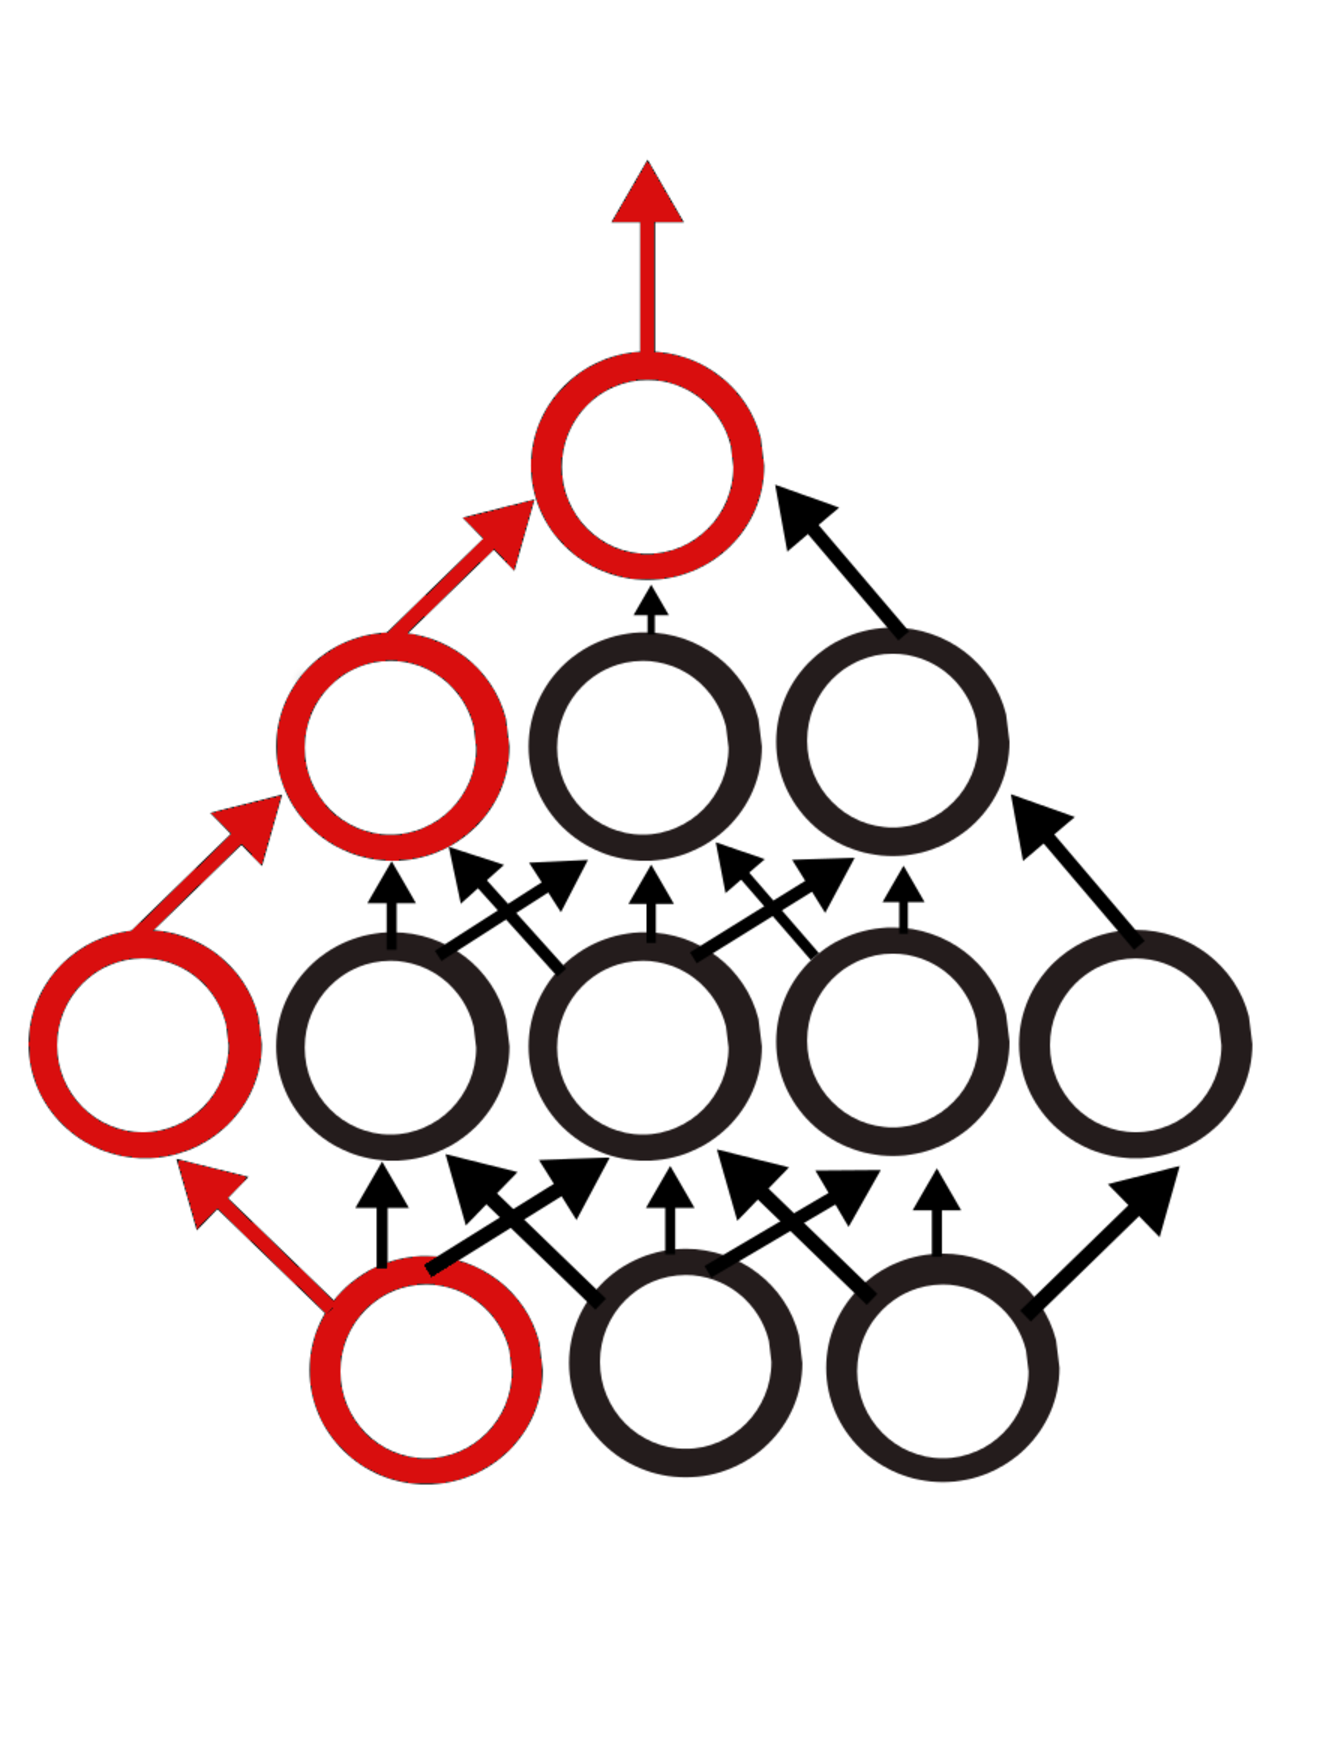
\includegraphics[width=\linewidth]{./Images/Chapter06/random_ticket_1.pdf}
\endminipage
\caption{A visual representation of the LTH as introduced by \citet{frankle2018lottery}. Let us consider a simplified version of a two hidden layer feedforward neural network as is depicted in the first image on the left. The LTH states that within this neural network, there exist multiple smaller networks (represented in green), which can perform just as well as their larger counterpart. Training these sparse models from scratch successfully is only possible as long as their weights are initialized with the same values that were also used when the larger (black) model was initialized. Furthermore, the structure of these sparse models appears to be crucial as well, as it is not possible to randomly extract any subset of weights from an unpruned model and successfully train the resulting sparse network (represented in red in the last figure) from scratch. We visually represent the performance of models that are the winners of the LTH in the two plots reported in Figure \ref{fig:original_lth_results}.} 
\label{fig:tickets_visualization}
\end{figure*}

\begin{figure}[ht!]
  \centering
  \begin{tikzpicture}[scale = 0.5]

\begin{axis}[
	grid style={dashed,gray},
	grid = both, 
	tick style=black,
	x label style={at={(axis description cs:0.5,-0.1)},anchor=north},
  	xlabel=Fraction of Weights Pruned,
  	ylabel= Accuracy ($\%$),
	title=MNIST,
	%width=1,
	xtick=data,
	%xticklabels from table={../logs/mnist_example.txt}{pruning_stages},
	label style={font=\scriptsize},
	xticklabels = {0.0,0.2,0.36,0.488,0.59,0.672,0.738,0.79,0.832,0.866,0.893,0.914,0.931,0.945,0.956,0.965,0.972,0.977,0.982,0.986,0.988,0.991,0.993,0.994,0.995,0.996,0.997,0.998,0.998,0.998,0.999},
	x=4.5mm,
	ymin=85,
    	ymax=99,
	scale only axis,
	xticklabel style={rotate=90},
        %log ticks with fixed point,
        scaled ticks=true,
	/pgf/number format/fixed,
        %log ticks with fixed point,
  	legend pos=outer north east,
]

	\addlegendentry{Baseline}
	\addlegendentry{Winning Ticket $f(x;m\odot\theta_0)$}
	\addlegendentry{Random Ticket $f(x;m\odot\theta_r)$}

\addplot [ultra thick, black, mark=x] table [x expr=\coordindex, y=baseline]{./Results/Chapter06/logs/mnist_example.txt};

\addplot [ultra thick, blue, mark=x] table [x expr=\coordindex, y=ticket]{./Results/Chapter06/logs/mnist_example.txt};
%\addplot [name path=upper,draw=none] table[x expr=\coordindex,y expr=\thisrow{ticket}+\thisrow{std-ticket}] {./Results/Chapter06/logs/mnist_example.txt};
%\addplot [name path=lower,draw=none] table[x expr=\coordindex,y expr=\thisrow{ticket}-\thisrow{std-ticket}] {./Results/Chapter06/logs/mnist_example.txt};
%\addplot [fill=blue!10] fill between[of=upper and lower];

\addplot [ultra thick, orange, mark=x] table [x expr=\coordindex, y=random_weights]{./Results/Chapter06/logs/mnist_example.txt};

\end{axis}
    \end{tikzpicture}
  \begin{tikzpicture}[scale = 0.5]

\begin{axis}[
	grid style={dashed,gray},
	grid = both, 
	tick style=black,
	x label style={at={(axis description cs:0.5,-0.1)},anchor=north},
  	xlabel=Fraction of Weights Pruned,
  	ylabel= Accuracy ($\%$),
	title=CIFAR-10,
	%width=1,
	xtick=data,
	label style={font=\scriptsize},
	xticklabels = {0.0,0.2,0.36,0.488,0.59,0.672,0.738,0.79,0.832,0.866,0.893,0.914,0.931,0.945,0.956,0.965,0.972,0.977,0.982,0.986,0.988,0.991,0.993,0.994,0.995,0.996,0.997,0.998,0.998,0.998,0.999},
	x=4.5mm,
	ymin=0,
    	ymax=90,
	scale only axis,
	xticklabel style={rotate=90},
        %log ticks with fixed point,
        scaled ticks=true,
	/pgf/number format/fixed,
        %log ticks with fixed point,
  	legend pos=outer north east,
]

	\addlegendentry{Baseline}
	\addlegendentry{Winning Ticket $f(x;m\odot\theta_k)$}
	\addlegendentry{Random Mask + Random $\theta$}

\addplot [ultra thick, black, mark=x] table [x expr=\coordindex, y=baseline]{./Results/Chapter06/logs/cifar10_example.txt};
\addplot [ultra thick, blue, mark=x] table [x expr=\coordindex, y=ticket]{./Results/Chapter06/logs/cifar10_example.txt};
\addplot [ultra thick, red, mark=x] table [x expr=\coordindex, y=random_mask]{./Results/Chapter06/logs/cifar10_example.txt};

\end{axis}
    \end{tikzpicture}


    \caption{A visual representation of the performance of lottery winners that replicate the findings first presented by \citet{frankle2018lottery}. In the first plot we consider a multilayer perceptron that gets trained on the MNIST dataset. After the network gets trained from scratch it obtains a final accuracy of $\approx 97\%$ as reported by the black line. We can observe that winning tickets $f(x;m\odot\theta_0)$ only start performing worse than the network they have been extracted from once a large fraction of their weights gets pruned. We can also observe how crucial it is to re-initialize the weights of the pruned models with the same weights that were used when initializing the unpruned model from scratch ($\theta_0$). If random weights are used instead ($\theta_r$), the pruned masks appear to be less robust to pruning (orange curve). In the second plot we show, for a  ResNet-50 architecture on the CIFAR-10 dataset, how important it is for a pruned model to come in the form of $f(x;m \odot\theta_k)$, where $\theta_k$ are the parameters obtained after $k$ training epochs ($k=2$ in this plot). Indeed, the red curve shows that it is not possible to simply extract any random subset of weights from a deep convolutional network and obtain a performance that is robust to pruning after randomly initializing the parameters of the model.}
    \label{fig:original_lth_results}
\end{figure} 


Since the introduction of the idea of the LTH, several research works have focused on understanding what makes some weights so special to be the winners of the initialization lottery. Among the different tested approaches, which will be reviewed in Sec. \ref{sec:related_work}, one research direction, in particular, has looked into how well winning ticket initializations can be transferred among different training settings (datasets and optimizers), an approach that aims at characterizing the winners of the LTH by studying to what extent their \textcolor{RoyalBlue}{inductive biases} are generic \cite{morcos2019one}. The most interesting findings of this study are that winning tickets generalize across datasets, within the natural image domain at least, and that tickets obtained from larger datasets typically generalize better. This opens the door to the transfer of winning tickets between datasets, which makes the high computational cost required to identify them much more acceptable in practice, as this cost has to be paid only once and can be shared across datasets.

In this chapter, we build on top of this latter work. While \citet{morcos2019one} focused on the natural image domain, we investigate the possibility of transferring winning tickets obtained from the natural image domain to datasets in non-natural image domains. This question has an important practical interest as datasets in non-natural image domains are typically scarcer than datasets in natural image domains. They would, therefore, potentially benefit more from a successful transfer of sparse networks since the latter can be expected to require less data for training than large over-parametrized networks. Furthermore, besides studying their generalization capabilities, we also focus on another interesting property that characterizes models that win the LTH, and which so far has received less research attention. As originally presented by \citet{frankle2018lottery}, pruned models, which are the winners of the LTH, can yield a final performance that is better than the one obtained by larger over-parametrized networks. In this chapter we explore whether it is worth seeking such pruned models when training data is scarce, a scenario that is well known to constraint the training of deep neural networks. To answer these two questions, we carried out experiments on several datasets from two very different non-natural image domains: digital pathology and, similarly to Chapters \ref{ch:tl_natural_to_non_natural} and \ref{ch:minerva}, digital heritage.

\section{Datasets}
\label{sec:datasets}

We consider seven datasets that will serve as target domains $\mathcal{D}_T$, and that come from two different, unrelated sources: histopathology and digital heritage. Each dataset comes with its training, validation, and testing splits. Furthermore, the datasets change in size, resolution, and amount of labels that need to be classified. We report an overview about the size of these datasets in Table \ref{tab:lth_datasets} while a visual representation of the samples constituting these datasets in Fig. \ref{fig:dataset_images}.
The Digital-Pathology (DP) data comes from the \texttt{Cytomine} \cite{maree2016collaborative} web application, the same open-source platform that allowed the creation of the MINERVA dataset described in the previous chapter. While \texttt{Cytomine} has collected many datasets over the years, in what follows, we have limited our analysis to a subset of four datasets that all represent tissues and cells from either human or animal organs. These datasets, which therefore correspond to the first four target tasks $\mathcal{T}_T$ that will be considered throughout this chapter are: \texttt{Human-LBA}, \texttt{Lung-Tissues}, and \texttt{Mouse-LBA} (which were originally proposed in \cite{mormont2018comparison}), and \texttt{Bone-Marrow} (which comes from \cite{kainz2017training}). All four datasets have been used by \citet{mormont2018comparison}, who, as described in Chapter \ref{ch:transfer_learning}, researched whether neural networks pre-trained on natural images could successfully be re-used in the DP domain. In this chapter, we explore whether an alternative to their transfer-learning approaches could be based on training pruned networks that are the winners of the LTH. This will allow us to investigate the two research questions introduced in Sec. \ref{sec:intro}: we will explore whether winning initializations that are found on datasets of natural images do generalize to non-natural domains and whether sparse models winners of the LTH can perform better than larger unpruned models that get trained from scratch. 
Regarding the field of Digital-Humanities (DH) we use three novel, small datasets that all revolve around the target task $\mathcal{T}_T$ that is the classification of artworks. We consider two different target tasks that were already studied in Chapter \ref{ch:tl_natural_to_non_natural}, namely type and artist classification. When it comes to the latter target task $\mathcal{T}_T$ we use two different datasets, referred to as \textt{Artist} \circled{1} and \textt{Artist} \circled{2}, which purpose will be better explained in Sec. \ref{sec:additional_studies}. All images are publicly available as part of the WikiArt gallery \cite{phillips2011wiki} and can also be found within the large popular OmniArt dataset \cite{strezoski2018omniart}. Albeit as we have seen in Chapter \ref{ch:tl_natural_to_non_natural} in DH it is possible to find large datasets, which cannot be said for the field of histopathology, it is worth mentioning that we have kept the size of these datasets intentionally small in order to fit the research questions introduced in Sec. \ref{sec:intro}. 

\begin{table*}[ht]
\caption{A brief overview of the seven different datasets which have been used in this work. As usual throughout this thesis $N_t$ corresponds to the total amount of samples that are present in the dataset, while $Q_t$ represents the number of classes.}
\resizebox{\columnwidth}{!}{%
\centering
\begin{tabular}{lcccccc}
\hline
Dataset & Training-Set & Validation-Set & Testing-Set &$N_t$ & $Q_t$\\
\hline
\texttt{Human-LBA} &4051 &346 &1023 &5420 & 9  \\
\texttt{Lung-Tissues} &4881 &562 &888 &6331 & 10 \\
\texttt{Mouse-LBA} &1722 &716 &1846 &4284 & 8    \\
\texttt{Bone-Marrow} & 522 & 130 & 639 & 1291 & 8\\
\hline
\texttt{Artist-Classification-1} & 3103 & 389 & 389 & 3881 & 20\\
\texttt{Type-Classification} & 2868 & 360 & 360 & 3588 & 20 \\
\texttt{Artist-Classification-2} & 2827 & 353 & 353 & 3533 & 19\\
\hline
\end{tabular}%
}
\label{tab:lth_datasets}
\end{table*}


\begin{figure*}
  \centering
   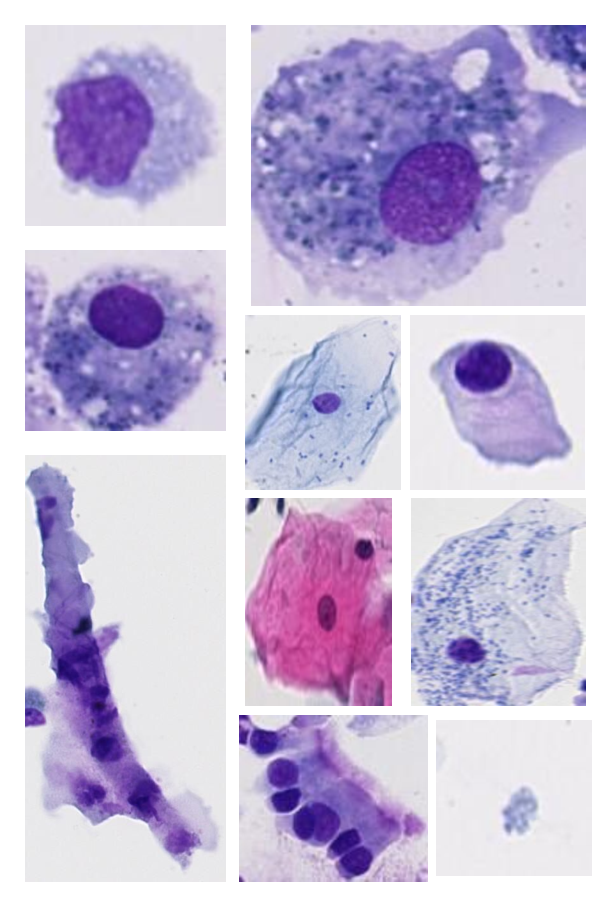
\includegraphics[width=2cm,height=\textheight,keepaspectratio]{./Images/Chapter06/lba.pdf}%
  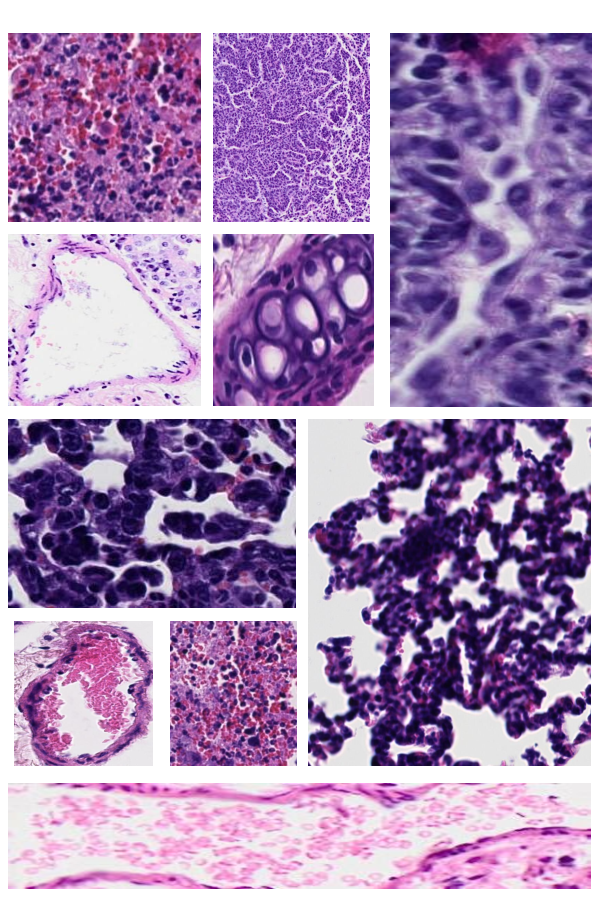
\includegraphics[width=2cm,height=\textheight,keepaspectratio]{./Images/Chapter06/tissus.pdf}%
  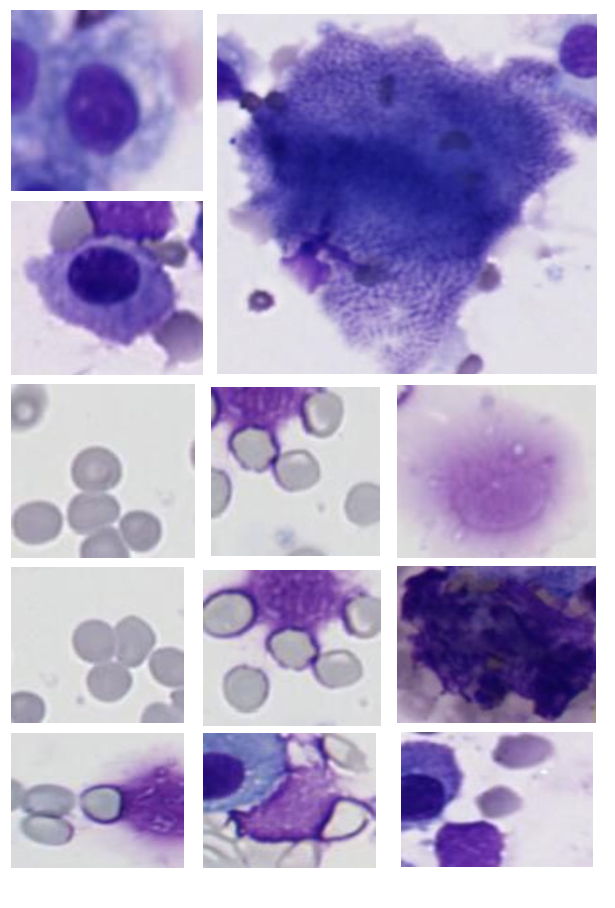
\includegraphics[width=2cm,height=\textheight,keepaspectratio]{./Images/Chapter06/mouse_lba.pdf}%
    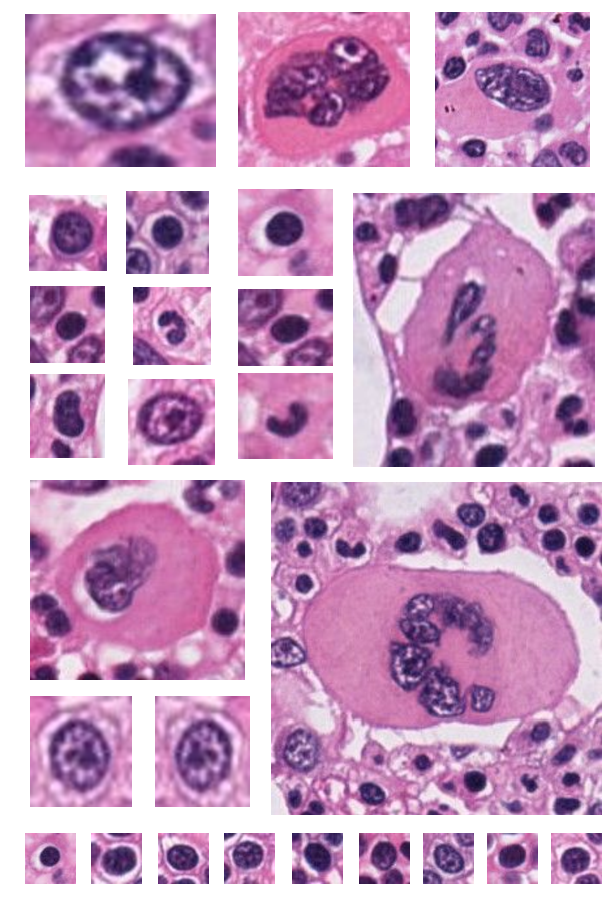
\includegraphics[width=2cm,height=\textheight,keepaspectratio]{./Images/Chapter06/bonemarrow.pdf}%
  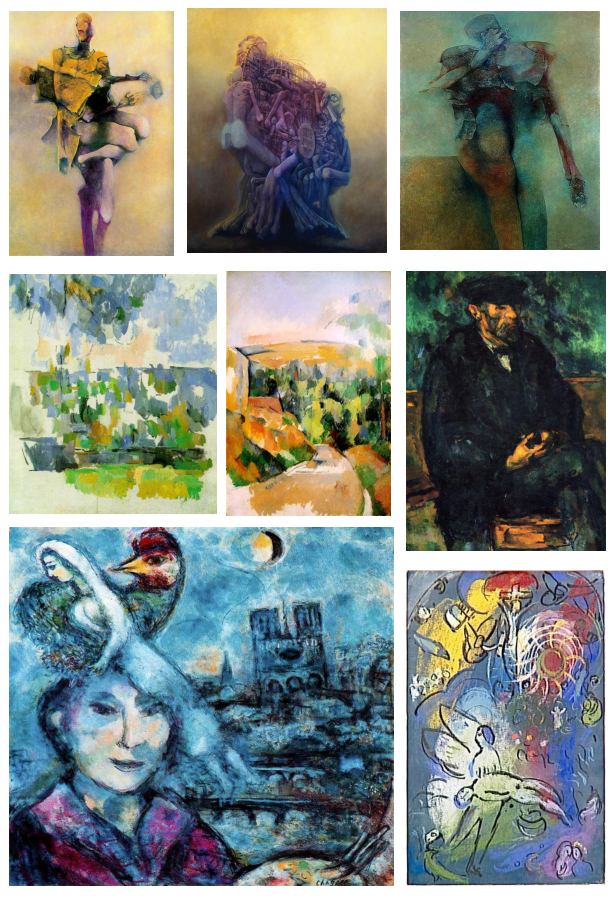
\includegraphics[width=2cm,height=\textheight,keepaspectratio]{./Images/Chapter06/artist.pdf}%
  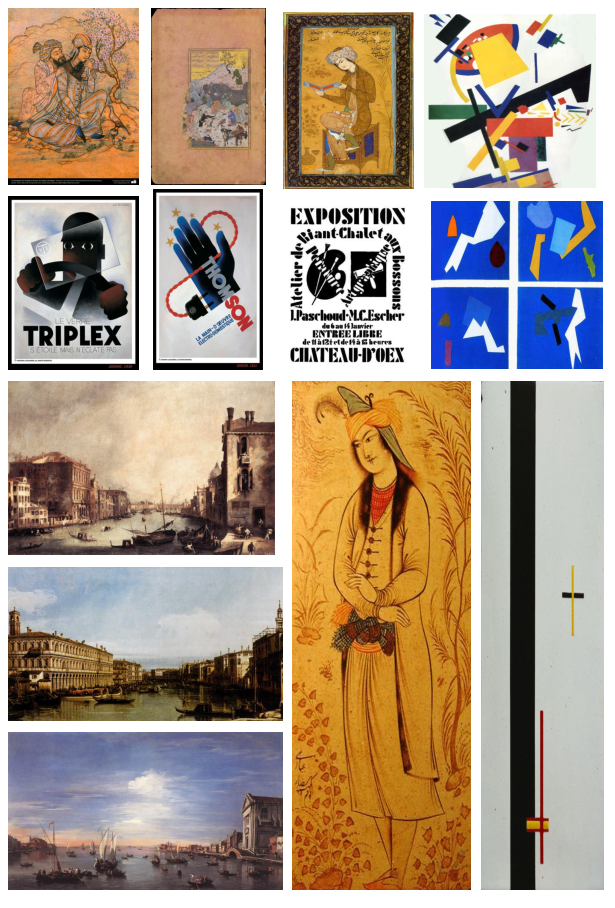
\includegraphics[width=2cm,height=\textheight,keepaspectratio]{./Images/Chapter06/type.pdf}%
  \caption{Some image samples that constitute the non-natural image datasets which have been used in this work. From left to right we have the \texttt{Human-LBA}, \texttt{Lung-Tissues}, \texttt{Mouse-LBA} and \texttt{Bone-Marrow} datasets, while finally we report some examples that represent artworks which come from the field of digital heritage and that are therefore similar to the images we have used for the experiments reported in Chapters \ref{ch:tl_natural_to_non_natural} and \ref{ch:minerva}.}
\label{fig:dataset_images}
\end{figure*}

\section{Experimental Setup}
\label{sec:experimental_setup}
We follow an experimental set-up similar to the one that was introduced in \cite{morcos2019one} (and that has been validated by \citet{gohil2019one}).
Let us define a neural network $f(x;\theta)$ that gets randomly initialized with parameters $\theta_0 \sim \mathscr{D}_{\theta}$ and then trained for $j$ iterations
over an input space $\mathcal{X}$, and an output space $\mathcal{Y}$. 
At the end of training a percentage of the parameters in $\theta_j$ gets pruned, a procedure which results in a mask $m$. The parameters in $\theta_j$ which did not get pruned are then reset to the values they had at $\theta_k$, where $k$ represents an early training iteration. A winning ticket corresponds to the combination between the previously obtained mask, and the parameters $\theta_k$, and is defined as $f(x;m\odot\theta_k)$ \footnote{Note that this formulation generalizes the original version of the LTH \cite{frankle2018lottery} that we have represented in Fig. \ref{fig:tickets_visualization}, where a winning ticket is obtained after resetting the unpruned parameters of the network to the values they had right after initialization, therefore defining a winning ticket as $f(x;m\odot\theta_0)$.}. Constructing a winning ticket with parameters $\theta_k$, instead of $\theta_0$, is a procedure which is known as late-resetting \cite{franklestabilizing}, and is a simple but effective trick that makes it possible to stably find winning initializations in deep convolutional neural networks \cite{franklestabilizing,morcos2019one}. In this study $f(x;\theta)$ comes in the form of a ResNet-50 architecture \cite{han2015deep} which gets trained on three popular CV natural image datasets serving as source domains $\mathcal{D}_S$: CIFAR-10/100 and Fashion-MNIST (see Fig. \ref{fig:natural_source_datasets} for a visualization). Following \cite{han2015deep,morcos2019one}, 31 winning tickets $f(x;m\odot\theta_k)$ of increasing sparsity are obtained from each of these three datasets by repeating 31 iterations of network training and magnitude pruning with a pruning rate $p$ of 20\%. Specifically, given a tensor $\mathbf{T}$ representing the unpruned parameters in a layer, at each pruning iteration we first train the network for several epochs (using early stopping on the validation set as described in the appendix), and then remove all entries in channel $c$ along dimension $d$ as:
\begin{equation}
  \Big\{\mathbf{T}_{[..., c, ...]} : c_{\text{th}} \Big\( \{\mathbf{T}_{[..., i, ...]}\}^{d}_{i=1} ||\cdot||_1 \Big\) \leq p \Big\},
\end{equation}
\label{eq:magnitude_pruning}
where $k_{\text{th}}$ is the rank of the $k^{\text{th}}$ channel of $\mathbf{T}$ along direction $d$ according to the $L_1$-based ranking \cite{paganini2020bespoke}.
The parameters $\theta_k$ that define each of the 31 tickets are then taken as the weights of the corresponding pruned networks at the $k$th epoch of the first pruning iteration. Once these pruned networks are found, we aim at investigating whether their parameters $\theta_k$ contain inductive biases that allow them to generalize to the non-natural image domain. To do so, we replace the final fully connected layer of each winning ticket with a randomly initialized layer that has as many output nodes as there are classes to classify. We then fine-tune each of these networks on the non-natural target tasks $\mathcal{T}_T$ considered in this study.
At the end of training, we study the performance of each winning ticket in two different ways. First, we compare the performance of each network to the performance of a fully unpruned network that gets randomly initialized and trained from scratch. Second, we also compare the performance of winning tickets that have been found on a natural image dataset to 31 new sparse models that are the winners of the LTH on the considered target dataset. Since it is not known to which extent pruned networks that contain weights that are the winners of the LTH on a natural image dataset can generalize to target domains $\mathcal{D}_T$ that do not contain natural images, we report the first results that investigate the potential of a novel transfer-learning scheme which has so far only been studied on datasets from the natural image domain. Moreover, testing the performance of sparse networks that contain winning tickets that are specific to a non-natural image target distribution also allows us to investigate whether it is worth pruning large networks with the hope of finding smaller models that might perform better than a large over-parametrized one. As mentioned in Sec. \ref{sec:intro}, pruned networks that are initialized with the winning weights can sometimes perform better than a fully unpruned network. Identifying such sparse networks leads to a very significant reduction of model size, which can be a very effective way of regularization when training data is scarce.

\begin{figure*}
  \centering
   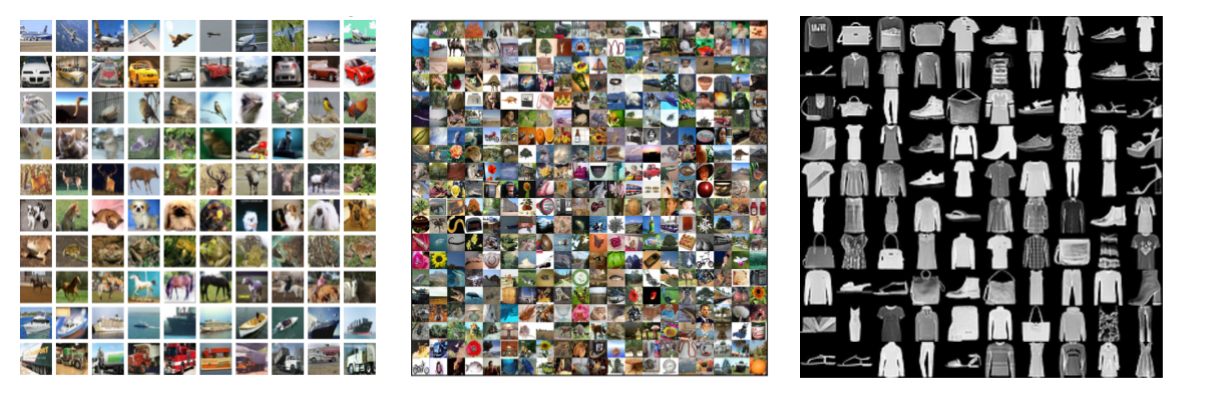
\includegraphics[width=\linewidth,height=\textheight,keepaspectratio]{./Images/Chapter06/natural_datasets.png}
   \caption{The three natural datasets constituting the source tasks $\mathcal{T}_S$ that are necessary for finding winning tickets. From left to right samples from the CIFAR-10/100 and Fashion-MNIST datasets.}
\label{fig:natural_source_datasets}
\end{figure*}


\section{Results}
\label{sec:results}
The results of all our experiments are visually reported in the plots of Fig. \ref{fig:tl_learning_with_lottery_tickets_results}. Each line plot represents the final performance obtained by a pruned model containing a winning ticket initialization on the final testing set of our target datasets. This performance is reported on the y-axis of the plots, while on the x-axis we represent the fraction of weights that are pruned from the original ResNet-50 architecture. As explained in the previous section, the performance of each winning ticket is compared to the performance obtained by an unpruned, over-parametrized architecture reported by the black dashed lines. The models that are the winners of the LTH on a natural image dataset are reported by the green, red and purple lines, while the blue lines report the winners of the LTH on a non-natural target dataset. Furthermore, when it comes to the latter lottery tickets, we also report the performance that is obtained by winning tickets that get randomly reinitialized ($f(x;m\odot\theta^{'}_{0})$ with $\theta^{'}_{0} \sim \mathscr{D}_\theta$). The orange lines report these results. 

\subsection{On the Importance of Finding Winning Initializations}
We can start by observing that pruned models which happen to be the winners of the LTH either on a natural dataset or on a non-natural one can maintain a good final performance until large pruning rates are reached. This is particularly evident on the first three datasets, where models that keep only $\approx 1\%$ of their original weights barely suffer from any drop in performance. This gets a little bit less evident on the last three datasets, where the performance of winning ticket initializations that are directly found on the considered target dataset starts getting harmed once a fraction of $\approx 97$ of original weights are pruned. These results show that an extremely large part of the parameters of a ResNet-50 architecture can be considered superfluous, therefore confirming the LTH when datasets contain non-natural images. More importantly, we also observe that pruned models winners of the LTH, significantly outperform larger over-parametrized models that get trained from scratch. This can be very clearly seen in all plots where the performance of pruned models is always consistently better than what is reported by the black dashed line. To get a better sense of how much these pruned networks perform better than their larger unpruned counterparts, we report in Table \ref{tab:results} the performance that is obtained by the best performing pruned model, found over all 31 possible pruned models, and compare it to the performance of an unpruned architecture. The exact fraction of weights which is pruned from an original ResNet-50 architecture is reported in Table \ref{tab:fraction_results} for each configuration. We can observe that no matter which dataset has been used as source domain $\mathcal{D}_S$ for finding a winning ticket initialization, all pruned networks reach a final accuracy that is significantly higher than the one that is obtained after training an unpruned model from scratch directly on the target task $\mathcal{T}_T$. While in most cases, the difference in terms of performance is of $\approx 10\%$ (see e.g., the \texttt{Human-LBA, Lung-Tissues} and the \texttt{Type} datasets), it is worth highlighting that there are other cases in which this difference is even larger. This is the case for the \texttt{Mouse-LBA} and \texttt{Artist} \circled{1} datasets where a winning ticket coming from the CIFAR-10 dataset performs more than $20\%$ better than a model trained from scratch. These results show that to maximize the performance of deep networks, it is always worth finding and training pruned models that are the winners of the LTH.

\begin{table*}[ht!]
\small
\caption{The results comparing the performance that is obtained on the testing-set by the best pruned model winner of the LTH, and an unpruned architecture trained from scratch. The overall best performing model is reported in a green cell, while the second best one in a yellow cell. We can observe that pruned models winners of the LTH perform significantly better than a larger over-parametrized architecture that gets trained from scratch. As can be seen by the results obtained on the \texttt{Mouse-LBA} and \texttt{Artist} 1 datasets the difference in terms of performance can be particularly large ($\approx 20\%$).}
\resizebox{\columnwidth}{!}{%
\centering
\begin{tabular}{lcccccc}
\hline
Target-Dataset & Scratch-Training & CIFAR-10 & CIFAR-100 & Fashion-MNIST & Target-Ticket \\
\hline \hline
\texttt{Human-LBA} & $71.85_{\pm 1.12}$ &\cellcolor{yellow!25}$79.17_{\pm1.85}$ &$76.97_{\pm0.73}$ &$77.32_{\pm1.85}$ &\cellcolor{green!25}$81.72_{\pm0.39}$\\
\texttt{Lung-Tissues} &$84.75_{\pm0.81}$ &\cellcolor{yellow!25}$88.90_{\pm1.97}$ &$87.61_{\pm0.90}$ & $87.61_{\pm0.11}$ & $\cellcolor{green!25}90.48_{\pm0.16}$\\
\texttt{Mouse-LBA} &$48.17_{\pm1.18}$ &\cellcolor{green!25}$74.20_{\pm2.04}$ &$57.42_{\pm0.48}$ &$52.27_{\pm1.73}$ &\cellcolor{yellow!25}$68.20_{\pm3.79}$\\
\texttt{Bone-Marrow} &$64.66_{\pm1.36}$ &\cellcolor{yellow!25}$71.75_{\pm3.36}$ &$69.87_{\pm0.39}$&$68.77_{\pm0.39}$&$\cellcolor{green!25}72.55_{\pm0.46}$\\
\hline
\texttt{Artist} \circled{1} & $45.88_{\pm0.42}$ & $\cellcolor{green!25}66.58_{\pm1.54}$ & $\cellcolor{yellow!25}65.55_{\pm1.79}$ & $63.88_{\pm0.12}$ & $58.74_{\pm1.92}$\\
\texttt{Type} &$41.36_{\pm2.31}$ & $58.63_{\pm2.97}$ & $\cellcolor{green!25}60.56_{\pm0.44}$ & $\cellcolor{yellow!25}58.92_{\pm0.59}$ & $50.44_{\pm2.23}$ \\

\hline
\end{tabular}%
}
\label{tab:results}
\end{table*}

\begin{table*}[ht!]
\small
\caption{Some additional information about the lottery winners which performance is reported in Table \ref{tab:results}. For each winning ticket we report the fraction of weights that is pruned from an original ResNet-50 architecture and that therefore characterizes the level of sparsity of the overall best performing lottery ticket. The results in the Scratch-Training column are not reported as these are unpruned models that are trained from scratch.}
\resizebox{\columnwidth}{!}{%
\centering
\begin{tabular}{lccccc }
\hline
Target-Dataset & Scratch-Training & CIFAR-10 & CIFAR-100 & Fashion-MNIST & Target-Ticket \\
\hline \hline
\texttt{Human-LBA} & - & 0.945  & 0.79 & 0.886 & 0.832\\
\texttt{Lung-Tissues} & - & 0.977 & 0.977 & 0.672 &  0.965\\
\texttt{Mouse-LBA} & - & 0.972 & 0.893 & 0.738 & 0.931\\
\texttt{Bone-Marrow} & - & 0.866 & 0.988 & 0.931 & 0.914\\
\hline
\texttt{Artist} \circled{1} & - & 0.972 & 0.993 & 0.991 & 0.931\\
\texttt{Type} & - & 0.991 & 0.931 & 0.995 & 0.963\\

\hline
\end{tabular}%
}
\label{tab:fraction_results}
\end{table*}

\begin{figure}[ht!]
\centering
	\begin{tikzpicture}[scale = 0.45]

\begin{axis}[
	name=ax1,
	grid style={dashed,gray},
	grid = both, 
	tick style=black,
  	x label style={at={(axis description cs:0.5,-0.1)},anchor=north},
	xlabel=Fraction of Weights Pruned,
  	ylabel= Accuracy ($\%$),
	ylabel style={font=\Large},
	title=Human-LBA,
	xtick=data,
	label style={font=\scriptsize},
	xticklabels = {0.0,0.2,0.36,0.488,0.59,0.672,0.738,0.79,0.832,0.866,0.893,0.914,0.931,0.945,0.956,0.965,0.972,0.977,0.982,0.986,0.988,0.991,0.993,0.994,0.995,0.996,0.997,0.998,0.998,0.998,0.999},
	x=4.5mm,
	ymin=40,
    	ymax=90,
	scale only axis,
	xticklabel style={rotate=90},
        %log ticks with fixed point,
        scaled ticks=true,
	/pgf/number format/fixed,
        %log ticks with fixed point,
]

	%\addlegendentry{Baseline}
	%\addlegendentry{Winning Ticket $f(x;m\odot\theta_k)$}
	%\addlegendentry{Random Ticket $f(x;m\odot\theta_r)$}
	%\addlegendentry{CIFAR-10}
	%\addlegendentry{CIFAR-100}
	%\addlegendentry{Fashion-MNIST}


\addplot [thick, black, mark=x] table [x expr=\coordindex, y=baseline]{./Results/Chapter06/logs/human_lba.txt};
\addplot [thick, blue, mark=x] table [x expr=\coordindex, y=winning_ticket]{./Results/Chapter06/logs/human_lba.txt};
\addplot [thick, orange, mark=x] table [x expr=\coordindex, y=random_mask]{./Results/Chapter06/logs/human_lba.txt};
\addplot [thick, green, mark=x] table [x expr=\coordindex, y=cifar10]{./Results/Chapter06/logs/human_lba.txt};
\addplot [thick, red, mark=x] table [x expr=\coordindex, y=cifar100]{./Results/Chapter06/logs/human_lba.txt};
\addplot [thick, purple, mark=x] table [x expr=\coordindex, y=fahion_mnist]{./Results/Chapter06/logs/human_lba.txt};


%\legend{}
\end{axis}

\begin{axis}[
	at={(ax1.south east)},
	xshift=2cm,
	grid style={dashed,gray},
	grid = both, 
	tick style=black,
	x label style={at={(axis description cs:0.5,-0.1)},anchor=north},
  	xlabel=Fraction of Weights Pruned,
  	ylabel= Accuracy ($\%$),
	title=Lung Tissues,
	%width=1,
	xtick=data,
	label style={font=\scriptsize},
	xticklabels = {0.0,0.2,0.36,0.488,0.59,0.672,0.738,0.79,0.832,0.866,0.893,0.914,0.931,0.945,0.956,0.965,0.972,0.977,0.982,0.986,0.988,0.991,0.993,0.994,0.995,0.996,0.997,0.998,0.998,0.998,0.999},
	x=4.5mm,
	ymin=70,
    	ymax=95,
	scale only axis,
	xticklabel style={rotate=90},
        %log ticks with fixed point,
        scaled ticks=true,
	/pgf/number format/fixed,
        %log ticks with fixed point,
  	legend pos=outer north east,
	legend style={font=\small, at={(-0.8,-0.2,-0.2)},anchor=north west, legend columns = 1}
	]

	%\addlegendentry{Baseline}
	%\addlegendentry{Winning Ticket $f(x;m\odot\theta_k)$}
	%\addlegendentry{Random Ticket $f(x;m\odot\theta_r)$}
	%\addlegendentry{CIFAR-10}
	%\addlegendentry{CIFAR-100}
	%\addlegendentry{Fashion-MNIST}


\addplot [thick, black, mark=x] table [x expr=\coordindex, y=baseline]{./Results/Chapter06/logs/lung_tissues.txt};
\addplot [thick, blue, mark=x] table [x expr=\coordindex, y=winning_ticket]{./Results/Chapter06/logs/lung_tissues.txt};
\addplot [thick, orange, mark=x] table [x expr=\coordindex, y=random_mask]{./Results/Chapter06/logs/lung_tissues.txt};
\addplot [thick, green, mark=x] table [x expr=\coordindex, y=cifar10]{./Results/Chapter06/logs/lung_tissues.txt};
\addplot [thick, red, mark=x] table [x expr=\coordindex, y=cifar100]{./Results/Chapter06/logs/lung_tissues.txt};
\addplot [thick, purple, mark=x] table [x expr=\coordindex, y=fahion_mnist]{./Results/Chapter06/logs/lung_tissues.txt};

\end{axis}

\begin{axis}[
	at={(ax1.south east)},
	xshift=-10.7cm,
	yshift=-10cm,
	grid style={dashed,gray},
	grid = both, 
	tick style=black,
	x label style={at={(axis description cs:0.5,-0.1)},anchor=north},
  	xlabel=Fraction of Weights Pruned,
  	ylabel= Accuracy ($\%$),
	title=Mouse-LBA,
	%width=1,
	xtick=data,
	label style={font=\scriptsize},
	xticklabels = {0.0,0.2,0.36,0.488,0.59,0.672,0.738,0.79,0.832,0.866,0.893,0.914,0.931,0.945,0.956,0.965,0.972,0.977,0.982,0.986,0.988,0.991,0.993,0.994,0.995,0.996,0.997,0.998,0.998,0.998,0.999},
	x=4.5mm,
	ymin=0,
    	ymax=90,
	scale only axis,
	xticklabel style={rotate=90},
        %log ticks with fixed point,
        scaled ticks=true,
	/pgf/number format/fixed,
        %log ticks with fixed point,
  	%legend pos=outer north east,
	%legend style={font=\small, at={(-0.8,-0.2,-0.2)},anchor=north west, legend columns = 1}
	]

	%\addlegendentry{Baseline}
	%\addlegendentry{Winning Ticket $f(x;m\odot\theta_k)$}
	%\addlegendentry{Random Ticket $f(x;m\odot\theta_r)$}
	%\addlegendentry{CIFAR-10}
	%\addlegendentry{CIFAR-100}
	%\addlegendentry{Fashion-MNIST}


\addplot [thick, black, mark=x] table [x expr=\coordindex, y=baseline]{./Results/Chapter06/logs/mouse_lba.txt};
\addplot [thick, blue, mark=x] table [x expr=\coordindex, y=winning_ticket]{./Results/Chapter06/logs/mouse_lba.txt};
\addplot [thick, orange, mark=x] table [x expr=\coordindex, y=random_mask]{./Results/Chapter06/logs/mouse_lba.txt};
\addplot [thick, green, mark=x] table [x expr=\coordindex, y=cifar10]{./Results/Chapter06/logs/mouse_lba.txt};
\addplot [thick, red, mark=x] table [x expr=\coordindex, y=cifar100]{./Results/Chapter06/logs/mouse_lba.txt};
\addplot [thick, purple, mark=x] table [x expr=\coordindex, y=fahion_mnist]{./Results/Chapter06/logs/mouse_lba.txt};

\end{axis}
    
\begin{axis}[
	at={(ax1.south east)},
	xshift=2cm,
	yshift=-10cm,
	grid style={dashed,gray},
	grid = both, 
	tick style=black,
	x label style={at={(axis description cs:0.5,-0.1)},anchor=north},
  	xlabel=Fraction of Weights Pruned,
  	ylabel= Accuracy ($\%$),
	title=Bone Marrow,
	%width=1,
	xtick=data,
	label style={font=\scriptsize},
	xticklabels = {0.0,0.2,0.36,0.488,0.59,0.672,0.738,0.79,0.832,0.866,0.893,0.914,0.931,0.945,0.956,0.965,0.972,0.977,0.982,0.986,0.988,0.991,0.993,0.994,0.995,0.996,0.997,0.998,0.998,0.998,0.999},
	x=4.5mm,
	ymin=20,
    	ymax=80,
	scale only axis,
	xticklabel style={rotate=90},
        %log ticks with fixed point,
        scaled ticks=true,
	/pgf/number format/fixed,
        %log ticks with fixed point,
  	%legend pos=outer north east,
	%legend style={font=\small, at={(-0.8,-0.2,-0.2)},anchor=north west, legend columns = 1}
	]

	%\addlegendentry{Baseline}
	%\addlegendentry{Winning Ticket $f(x;m\odot\theta_k)$}
	%\addlegendentry{Random Ticket $f(x;m\odot\theta_r)$}
	%\addlegendentry{CIFAR-10}
	%\addlegendentry{CIFAR-100}
	%\addlegendentry{Fashion-MNIST}


\addplot [thick, black, mark=x] table [x expr=\coordindex, y=baseline]{./Results/Chapter06/logs/bone_marrow.txt};
\addplot [thick, blue, mark=x] table [x expr=\coordindex, y=winning_ticket]{./Results/Chapter06/logs/bone_marrow.txt};
\addplot [thick, orange, mark=x] table [x expr=\coordindex, y=random_mask]{./Results/Chapter06/logs/bone_marrow.txt};
\addplot [thick, green, mark=x] table [x expr=\coordindex, y=cifar10]{./Results/Chapter06/logs/bone_marrow.txt};
\addplot [thick, red, mark=x] table [x expr=\coordindex, y=cifar100]{./Results/Chapter06/logs/bone_marrow.txt};
\addplot [thick, purple, mark=x] table [x expr=\coordindex, y=fahion_mnist]{./Results/Chapter06/logs/bone_marrow.txt};

\end{axis}
 
\begin{axis}[
	at={(ax1.south east)},
	xshift=-10.7cm,
	yshift=-20cm,
	grid style={dashed,gray},
	grid = both, 
	tick style=black,
	x label style={at={(axis description cs:0.5,-0.1)},anchor=north},
  	xlabel=Fraction of Weights Pruned,
  	ylabel= Accuracy ($\%$),
	title=Artist Classification 1,
	%width=1,
	xtick=data,
	label style={font=\scriptsize},
	xticklabels = {0.0,0.2,0.36,0.488,0.59,0.672,0.738,0.79,0.832,0.866,0.893,0.914,0.931,0.945,0.956,0.965,0.972,0.977,0.982,0.986,0.988,0.991,0.993,0.994,0.995,0.996,0.997,0.998,0.998,0.998,0.999},
	x=4.5mm,
	ymin=0,
    	ymax=75,
	scale only axis,
	xticklabel style={rotate=90},
        %log ticks with fixed point,
        scaled ticks=true,
	/pgf/number format/fixed,
        %log ticks with fixed point,
  	%legend pos=outer north east,
	%legend style={font=\small, at={(-0.8,-0.2,-0.2)},anchor=north west, legend columns = 1}
	]

	\addlegendentry{Baseline}
	\addlegendentry{Winning Ticket $f(x;m\odot\theta_k)$}
	\addlegendentry{Random Ticket $f(x;m\odot\theta_r)$}
	\addlegendentry{CIFAR-10}
	\addlegendentry{CIFAR-100}
	\addlegendentry{Fashion-MNIST}


\addplot [thick, black, mark=x] table [x expr=\coordindex, y=baseline]{./Results/Chapter06/logs/artist_classification_1.txt};
\addplot [thick, blue, mark=x] table [x expr=\coordindex, y=winning_ticket]{./Results/Chapter06/logs/artist_classification_1.txt};
\addplot [thick, orange, mark=x] table [x expr=\coordindex, y=random_mask]{./Results/Chapter06/logs/artist_classification_1.txt};
\addplot [thick, green, mark=x] table [x expr=\coordindex, y=cifar10]{./Results/Chapter06/logs/artist_classification_1.txt};
\addplot [thick, red, mark=x] table [x expr=\coordindex, y=cifar100]{./Results/Chapter06/logs/artist_classification_1.txt};
\addplot [thick, purple, mark=x] table [x expr=\coordindex, y=fahion_mnist]{./Results/Chapter06/logs/artist_classification_1.txt};

\legend{}
\end{axis}
    
\begin{axis}[
	at={(ax1.south east)},
	xshift=2cm,
	yshift=-20cm,
	grid style={dashed,gray},
	grid = both, 
	tick style=black,
	x label style={at={(axis description cs:0.5,-0.1)},anchor=north},
  	xlabel=Fraction of Weights Pruned,
  	ylabel= Accuracy ($\%$),
	title=Type Classification,
	%width=1,
	xtick=data,
	label style={font=\scriptsize},
	xticklabels = {0.0,0.2,0.36,0.488,0.59,0.672,0.738,0.79,0.832,0.866,0.893,0.914,0.931,0.945,0.956,0.965,0.972,0.977,0.982,0.986,0.988,0.991,0.993,0.994,0.995,0.996,0.997,0.998,0.998,0.998,0.999},
	x=4.5mm,
	ymin=10,
    	ymax=70,
	scale only axis,
	xticklabel style={rotate=90},
        %log ticks with fixed point,
        scaled ticks=true,
	/pgf/number format/fixed,
        %log ticks with fixed point,
  	legend pos=outer north east,
	legend style={font=\Large, at={(-0.8,-0.35,-0.2)},anchor=north west, legend columns = 2}
	]

	\addlegendentry{Baseline}
	\addlegendentry{Winning Ticket $f(x;m\odot\theta_k)$}
	\addlegendentry{Random Ticket $f(x;m\odot\theta_r)$}
	\addlegendentry{CIFAR-10}
	\addlegendentry{CIFAR-100}
	\addlegendentry{Fashion-MNIST}


\addplot [thick, black, mark=x] table [x expr=\coordindex, y=baseline]{./Results/Chapter06/logs/type_classification.txt};
\addplot [thick, blue, mark=x] table [x expr=\coordindex, y=winning_ticket]{./Results/Chapter06/logs/type_classification.txt};
\addplot [thick, orange, mark=x] table [x expr=\coordindex, y=random_mask]{./Results/Chapter06/logs/type_classification.txt};
\addplot [thick, green, mark=x] table [x expr=\coordindex, y=cifar10]{./Results/Chapter06/logs/type_classification.txt};
\addplot [thick, red, mark=x] table [x expr=\coordindex, y=cifar100]{./Results/Chapter06/logs/type_classification.txt};
\addplot [thick, purple, mark=x] table [x expr=\coordindex, y=fahion_mnist]{./Results/Chapter06/logs/type_classification.txt};

\end{axis} 


    \end{tikzpicture}


   \caption{An overview of the results showing that sparse models that are the winners of the LTH (represented by the coloured lines) significantly outperform unpruned networks which get randomly initialized and trained from scratch (dashed black line). This happens to be the case on all tested datasets, no matter whether a winning initialization comes from a natural image source or not. It is however worth mentioning that, especially on the biomedical datasets, natural image tickets get outperformed by sparse networks that that are the winners of the LTH on a biomedical dataset. On the other hand this is not the case when it comes to the classification of arts where natural image tickets outperform the ones which are found within artistic collections.}
    \label{fig:tl_learning_with_lottery_tickets_results}
\end{figure} 



\subsection{On the Generalization Properties of Lottery Winners}
We then investigate whether natural image tickets can generalize to the non-natural setting, therefore accounting for the distribution shift between domains $\mathcal{D}$. Findings differ across datasets. When considering the datasets that come from the DP field, we can see that, in three out of four cases, winning tickets that are found on a natural image dataset get outperformed by sparse winning networks that come after training a model on the biomedical dataset. This is particularly evident in the results obtained on the \texttt{Human-LBA} and \texttt{Lung-Tissues} datasets, where the blue line plots consistently reach the highest testing-set accuracy. When it comes to the \texttt{Bone-Marrow} dataset, the difference in terms of performance between the best natural image ticket, in this case coming from the CIFAR-10 dataset, and the one coming from the biomedical dataset, is less evident (see Table \ref{tab:results} for the exact accuracies). Furthermore, it is worth highlighting that on the \texttt{Bone-Marrow} dataset, albeit natural image models seem to get outperformed by the ones found on the biomedical dataset, the performance of the latter ones appears to be less stable once substantial pruning rates are reached. When it comes to the \texttt{Mouse-LBA} dataset, these results slightly differ. In fact, this dataset corresponds to the only case where a natural image source ticket outperforms a non-natural one. As can be seen, by the green line plot, pruned models coming from the CIFAR-10 dataset outperform the ones found on the \texttt{Mouse-LBA} dataset. 

When focusing our analysis on the classification of arts, we see that the results change significantly from the ones obtained on the biomedical datasets. In this case, all of the natural image lottery winners, no matter the source tasks $\mathcal{D}_S$ they were initially found on, outperform the same kind of models that were found after training a full network on the artistic collection. We can see from Table \ref{tab:results} that the final testing performance is similar among all of the best natural image tickets. Similar to what has been noticed on the \texttt{Bone-Marrow} dataset, we can again observe that tickets coming from a non-natural data distribution seem to suffer more from large pruning rates. 

These results show both the potential and limitations that natural image winners of the LTH can offer when fine-tuned on non-natural images datasets. The results obtained on the artistic datasets suggest that winning initializations contain inductive biases that are strong enough to get at least successfully transferred to the artistic domain, therefore confirming some of the claims that were made by \citet{morcos2019one}. However, it also appears that there are stronger limitations to the transferability of winning initializations which were not observed by \citet{morcos2019one}. In fact, our results show that on DP data, the best strategy is to find a winning ticket directly on the biomedical dataset, and that winning initializations found on natural image datasets, albeit outperforming a randomly initialized unpruned network, perform worse than pruned models that are the winners of the LTH on a biomedical dataset.

\section{Additional Studies}
\label{sec:additional_studies}
To characterize the transferability of winning initializations even more while at the same time gaining a deeper understanding of the LTH, we have performed a set of three additional experiments which help us characterize this phenomenon better. 

\subsubsection{Lottery Tickets VS fine-tuned pruned models}
So far, we have focused our transfer learning study on lottery tickets that come in the form of $f(x;m\odot\theta_k)$, where, as mentioned in Sec. \ref{sec:experimental_setup}, $\theta_k$ corresponds to the weights that parametrize a neural network at a very early training iteration. This formalization is, however, different from the transfer learning scenarios that we have described in Chapter \ref{ch:transfer_learning} and adapted in Chapters \ref{ch:tl_natural_to_non_natural} and \ref{ch:minerva}, where neural networks get transferred with the weights that are obtained at the end of the training process. We have therefore studied whether there is a difference in terms of performance between transferring and fine-tuning a lottery ticket with parameters $\theta_k$, and the same kind of pruned network which is initialized with the weights that are obtained once the network is fully trained on a source task $\mathcal{T}_S$. We define these kind of models as $f(x;m\odot\theta_i)$ where $i$ stays for the last training iteration. We report some examples of this behaviour in the plots presented in Fig. \ref{fig:full_fine_tuning_comparison}, where we consider $f(x;m\odot\theta_i)$ models which were trained on the CIFAR-10 and CIFAR-100 datasets, and then transferred and fine-tuned on the \texttt{Human-LBA} dataset. We found that these models overall perform worse than lottery tickets while also being less robust to pruning. This also shows that on this dataset, the slightly inferior performance of the natural image tickets with respect to the target tickets is not due to the weight re-initialization.

\begin{figure}[ht!]
\centering
	\begin{tikzpicture}[scale = 0.45]

\begin{axis}[
	name=ax1,
	grid style={dashed,gray},
	grid = both, 
	tick style=black,
  	x label style={at={(axis description cs:0.5,-0.1)},anchor=north},
	xlabel=Fraction of Weights Pruned,
  	ylabel= Accuracy ($\%$),
	title=Human-LBA,
	%width=1,
	xtick=data,
	label style={font=\scriptsize},
	xticklabels = {0.0,0.2,0.36,0.488,0.59,0.672,0.738,0.79,0.832,0.866,0.893,0.914,0.931,0.945,0.956,0.965,0.972,0.977,0.982,0.986,0.988,0.991,0.993,0.994,0.995,0.996,0.997,0.998,0.998,0.998,0.999},
	x=4.5mm,
	ymin=40,
    	ymax=90,
	scale only axis,
	xticklabel style={rotate=90},
        %log ticks with fixed point,
        scaled ticks=true,
	/pgf/number format/fixed,
        %log ticks with fixed point,
  	legend pos= north east,
	%legend style={font=\small, at={(-0.8,-0.2,-0.2)},anchor=north west, legend columns = 1}
	]

	\addlegendentry{Baseline}
	\addlegendentry{Winning Ticket $f(x;m\odot\theta_k)$}
	\addlegendentry{CIFAR-10 $f(x;m\odot\theta_i)$}
	
\addplot [thick, black, mark=x] table [x expr=\coordindex, y=baseline]{./Results/Chapter06/logs/human_lba_fine_tuning_study.txt};
\addplot [thick, green, mark=x] table [x expr=\coordindex, y=winning_ticket]{./Results/Chapter06/logs/human_lba_fine_tuning_study.txt};
\addplot [thick, green, mark=*] table [x expr=\coordindex, y=fine_tuned_pruned_model]{./Results/Chapter06/logs/human_lba_fine_tuning_study.txt};

\end{axis}
\end{tikzpicture}
\begin{tikzpicture}[scale = 0.45]
\begin{axis}[
	at={(ax1.south east)},
	xshift=2cm,
	grid style={dashed,gray},
	grid = both, 
	tick style=black,
	x label style={at={(axis description cs:0.5,-0.1)},anchor=north},
  	xlabel=Fraction of Weights Pruned,
  	ylabel= Accuracy ($\%$),
	title=Human-LBA,
	%width=1,
	xtick=data,
	label style={font=\scriptsize},
	xticklabels = {0.0,0.2,0.36,0.488,0.59,0.672,0.738,0.79,0.832,0.866,0.893,0.914,0.931,0.945,0.956,0.965,0.972,0.977,0.982,0.986,0.988,0.991,0.993,0.994,0.995,0.996,0.997,0.998,0.998,0.998,0.999},
	x=4.5mm,
	ymin=40,
    	ymax=90,
	scale only axis,
	xticklabel style={rotate=90},
        %log ticks with fixed point,
        scaled ticks=true,
	/pgf/number format/fixed,
        %log ticks with fixed point,
  	legend p= north east,
	%legend style={font=\Large, at={(-0.8,-0.2,-0.2)},anchor=north west, legend columns = 2}
	]

	\addlegendentry{Baseline}
	\addlegendentry{Winning Ticket $f(x;m\odot\theta_k)$}
	\addlegendentry{CIFAR-100 $f(x;m\odot\theta_i)$}
	
\addplot [thick, black, mark=x] table [x expr=\coordindex, y=baseline]{./Results/Chapter06/logs/human_lba_fine_tuning_study_cif.txt};
\addplot [thick, red, mark=x] table [x expr=\coordindex, y=winning_ticket]{./Results/Chapter06/logs/human_lba_fine_tuning_study_cif.txt};
	\addplot [thick, red, mark=*] table [x expr=\coordindex, y=fine_tuned_pruned_model]{./Results/Chapter06/logs/human_lba_fine_tuning_study_cif.txt};

\end{axis} 


    \end{tikzpicture}


    \caption{Our results showing the advantages of transferring lottery winners over pruned models that are fully fine-tuned on natural datasets (CIFAR-10/100). We can observe that their performance is overall inferior to the one of lottery tickets and that these models are significantly less robust to pruning. We believe that the reason behind their poor performance revolves around the fact that, once completely trained on a specific source task, and after having gone through the pruning stage, these models lose the necessary flexibility that is required for them to adapt to a new task.}
    \label{fig:full_fine_tuning_comparison}
\end{figure} 


\subsubsection{Transferring tickets from similar non-natural domains}
We investigated whether it is beneficial to fine-tune lottery winners that come from a natural image distribution instead of a related non-natural dataset. Specifically we tested whether winning tickets generated on the \texttt{Human-LBA} dataset generalize to the \texttt{Mouse-LBA} one (since both datasets are representative of the field of Live-Blood-Analysis), and whether lottery winners coming from the \texttt{Artist} \circled{1} dataset generalized to the \texttt{Artist} \circled{2} one. We visually represent these results in Fig. \ref{fig:from_similar_source_transfer}. As one might expect, we found that it is beneficial to transfer winning tickets from a related source. Specifically, \texttt{Human-LBA} tickets can perform just as well as winning tickets that are generated on the \texttt{Mouse-LBA} dataset, while at the same time also being more robust to large pruning rates. When it comes to lottery winners found on the \texttt{Artist} \circled{1} dataset we have observed that these tickets can even outperform the ones generated on the \texttt{Artist} \circled{2} one. Overall these results confirm the claims that we made in Chapter \ref{ch:tl_natural_to_non_natural} where we already highlighted the benefits that could come from transferring models that were trained on a similar source as the target task. This conclusion now also seems to hold for models that are the winners of the LTH. 

\begin{figure}[ht!]
\centering
	\begin{tikzpicture}[scale = 0.45]

\begin{axis}[
	name=ax1,
	grid style={dashed,gray},
	grid = both, 
	tick style=black,
  	x label style={at={(axis description cs:0.5,-0.1)},anchor=north},
	xlabel=Fraction of Weights Pruned,
  	ylabel= Accuracy ($\%$),
	title=Mouse-LBA,
	%width=1,
	xtick=data,
	label style={font=\scriptsize},
	xticklabels = {0.0,0.2,0.36,0.488,0.59,0.672,0.738,0.79,0.832,0.866,0.893,0.914,0.931,0.945,0.956,0.965,0.972,0.977,0.982,0.986,0.988,0.991,0.993,0.994,0.995,0.996,0.997,0.998,0.998,0.998,0.999},
	x=4.5mm,
	ymin=0,
    	ymax=90,
	scale only axis,
	xticklabel style={rotate=90},
        %log ticks with fixed point,
        scaled ticks=true,
	/pgf/number format/fixed,
        %log ticks with fixed point,
  	legend pos= north east,
	%legend style={font=\small, at={(-0.8,-0.2,-0.2)},anchor=north west, legend columns = 1}
	]

	\addlegendentry{Baseline}
	\addlegendentry{Winning Ticket $f(x;m\odot\theta_k)$}
	\addlegendentry{CIFAR-10}
	\addlegendentry{CIFAR-100}
	\addlegendentry{Fashion-MNIST}
	\addlegendentry{Related Ticket}


\addplot [thick, black, mark=x] table [x expr=\coordindex, y=baseline]{./Results/Chapter06/logs/from_lba_to_lba.txt};
\addplot [thick, blue, mark=x] table [x expr=\coordindex, y=winning_ticket]{./Results/Chapter06/logs/from_lba_to_lba.txt};
\addplot [thick, green, mark=x] table [x expr=\coordindex, y=cifar10]{./Results/Chapter06/logs/from_lba_to_lba.txt};
\addplot [thick, red, mark=x] table [x expr=\coordindex, y=cifar100]{./Results/Chapter06/logs/from_lba_to_lba.txt};
\addplot [thick, purple, mark=x] table [x expr=\coordindex, y=fahion_mnist]{./Results/Chapter06/logs/from_lba_to_lba.txt};
\addplot [thick, cyan, mark=x] table [x expr=\coordindex, y=similar_source]{./Results/Chapter06/logs/from_lba_to_lba.txt};


\legend{}
\end{axis}
\begin{axis}[
	at={(ax1.south east)},
	xshift=2cm,
	grid style={dashed,gray},
	grid = both, 
	tick style=black,
	x label style={at={(axis description cs:0.5,-0.1)},anchor=north},
  	xlabel=Fraction of Weights Pruned,
  	ylabel= Accuracy ($\%$),
	title=Artist 2,
	%width=1,
	xtick=data,
	label style={font=\scriptsize},
	xticklabels = {0.0,0.2,0.36,0.488,0.59,0.672,0.738,0.79,0.832,0.866,0.893,0.914,0.931,0.945,0.956,0.965,0.972,0.977,0.982,0.986,0.988,0.991,0.993,0.994,0.995,0.996,0.997,0.998,0.998,0.998,0.999},
	x=4.5mm,
	ymin=0,
    	ymax=80,
	scale only axis,
	xticklabel style={rotate=90},
        %log ticks with fixed point,
        scaled ticks=true,
	/pgf/number format/fixed,
        %log ticks with fixed point,
  	legend p= north east,
	legend style={font=\Large, at={(-0.8,-0.35,-0.2)},anchor=north west, legend columns = 2}
	]
	
	\addlegendentry{Baseline}
	\addlegendentry{Winning Ticket $f(x;m\odot\theta_k)$}
	\addlegendentry{CIFAR-10}
	\addlegendentry{CIFAR-100}
	\addlegendentry{Fashion-MNIST}
	\addlegendentry{Related Ticket}


	\addplot [thick, black, mark=x] table [x expr=\coordindex, y=baseline]{./Results/Chapter06/logs/from_artist_to_artist.txt};
	\addplot [thick, blue, mark=x] table [x expr=\coordindex, y=winning_ticket]{./Results/Chapter06/logs/from_artist_to_artist.txt};	
	\addplot [thick, green, mark=x] table [x expr=\coordindex, y=cifar10]{./Results/Chapter06/logs/from_artist_to_artist.txt};
	\addplot [thick, red, mark=x] table [x expr=\coordindex, y=cifar100]{./Results/Chapter06/logs/from_artist_to_artist.txt};
	\addplot [thick, purple, mark=x] table [x expr=\coordindex, y=fahion_mnist]{./Results/Chapter06/logs/from_artist_to_artist.txt};
	\addplot [thick, cyan, mark=x] table [x expr=\coordindex, y=similar_source]{./Results/Chapter06/logs/from_artist_to_artist.txt};

\end{axis} 


    \end{tikzpicture}


    \caption{Our results showing the benefits of transferring lottery winners that have been identified on a related source task. We can observe that on the \texttt{Mouse-LBA} dataset, winning tickets that were obtained on the \texttt{Human-LBA} dataset are the ones that are the most robust ones to pruning, while on the \texttt{Artist} 2 dataset we can observe that lottery winners that have been obtained on the \texttt{Artist} 1 dataset are both more robust to pruning, while they also yield overall better performance.}
    \label{fig:from_similar_source_transfer}
\end{figure} 



\subsubsection{On the size of the training set}
We have observed from the blue line plots of Fig. \ref{fig:tl_learning_with_lottery_tickets_results} that there are cases in which lottery winners are very robust to extremely large pruning rates (see as an example the first and second plots), while there are other cases in which their performance deteriorates faster with respect to the fraction of weights that get pruned. The most robust performance is obtained by winning tickets that are generated on the \texttt{Human-LBA} and \texttt{Lung-Tissues} datasets, which are the two target datasets that contain the largest amount of training samples. Therefore, we have studied whether there is a relationship between the size of the training data used for finding lottery winners and the robustness in terms of performance of the resulting pruned models. We generated lottery winners after incrementally reducing the size of the training data by $75\%$, $50\%$ and $25\%$, and then investigated whether we could observe a similar drop in performance like the one we have observed in the last three blue line-plots of Fig. \ref{fig:tl_learning_with_lottery_tickets_results} once a large fraction of weights got pruned. Perhaps surprisingly, we have observed that this was not the case, and as can be seen, by the plots represented in Fig. \ref{fig:training_data_study}, the performance of lottery winners that are found when using only $25\%$ of the training set is just as stable as the one of winning tickets which are generated on the entire dataset. However, it is worth mentioning that, albeit the performance of such sparse models is robust, their final performance on the testing set is lower than the one obtained by winning tickets that have been trained on the full training data distribution.

\begin{figure}[ht!]
\centering
	\begin{tikzpicture}[scale = 0.45]

\begin{axis}[
	name=ax1,
	grid style={dashed,gray},
	grid = both, 
	tick style=black,
  	x label style={at={(axis description cs:0.5,-0.1)},anchor=north},
	xlabel=Fraction of Weights Pruned,
  	ylabel= Accuracy ($\%$),
	title=Lung-Tissues,
	%width=1,
	xtick=data,
	label style={font=\scriptsize},
	xticklabels = {0.0,0.2,0.36,0.488,0.59,0.672,0.738,0.79,0.832,0.866,0.893,0.914,0.931,0.945,0.956,0.965,0.972,0.977,0.982,0.986,0.988,0.991,0.993,0.994,0.995,0.996,0.997,0.998,0.998,0.998,0.999},
	x=4.5mm,
	ymin=70,
    	ymax=95,
	scale only axis,
	xticklabel style={rotate=90},
        %log ticks with fixed point,
        scaled ticks=true,
	/pgf/number format/fixed,
        %log ticks with fixed point,
  	legend pos= north east,
	%legend style={font=\small, at={(-0.8,-0.2,-0.2)},anchor=north west, legend columns = 1}
	]

	\addlegendentry{Baseline}
	\addlegendentry{100\% of training data}
	\addlegendentry{75\% of training data}
	\addlegendentry{50\% of training data}
	\addlegendentry{25\% of training data}

\addplot [thick, black, mark=x] table [x expr=\coordindex, y=baseline]{./Results/Chapter06/logs/lung_tissues_percentage_study.txt};
\addplot [thick, blue, mark=x] table [x expr=\coordindex, y=100]{./Results/Chapter06/logs/lung_tissues_percentage_study.txt};
\addplot [thick, green, mark=x] table [x expr=\coordindex, y=75]{./Results/Chapter06/logs/lung_tissues_percentage_study.txt};
\addplot [thick, red, mark=x] table [x expr=\coordindex, y=50]{./Results/Chapter06/logs/lung_tissues_percentage_study.txt};
\addplot [thick, purple, mark=x] table [x expr=\coordindex, y=25]{./Results/Chapter06/logs/lung_tissues_percentage_study.txt};

\legend{}
\end{axis}
\begin{axis}[
	at={(ax1.south east)},
	xshift=2cm,
	grid style={dashed,gray},
	grid = both, 
	tick style=black,
	x label style={at={(axis description cs:0.5,-0.1)},anchor=north},
	y label style={font=\Large},
  	xlabel=Fraction of Weights Pruned,
  	ylabel= Accuracy ($\%$),
	title=Human-LBA,
	%width=1,
	xtick=data,
	label style={font=\scriptsize},
	xticklabels = {0.0,0.2,0.36,0.488,0.59,0.672,0.738,0.79,0.832,0.866,0.893,0.914,0.931,0.945,0.956,0.965,0.972,0.977,0.982,0.986,0.988,0.991,0.993,0.994,0.995,0.996,0.997,0.998,0.998,0.998,0.999},
	x=4.5mm,
	ymin=40,
    	ymax=90,
	scale only axis,
	xticklabel style={rotate=90},
        %log ticks with fixed point,
        scaled ticks=true,
	/pgf/number format/fixed,
        %log ticks with fixed point,
  	legend p= north east,
	legend style={font=\Large, at={(-0.8,-0.35,-0.2)},anchor=north west, legend columns = 3}
	]
	
	\addlegendentry{Baseline}
	\addlegendentry{100\% of training data}
	\addlegendentry{75\% of training data}
	\addlegendentry{50\% of training data}
	\addlegendentry{25\% of training data}

\addplot [thick, black, mark=x] table [x expr=\coordindex, y=baseline]{./Results/Chapter06/logs/human_lba_percentage_study.txt};
\addplot [thick, blue, mark=x] table [x expr=\coordindex, y=100]{./Results/Chapter06/logs/human_lba_percentage_study.txt};
\addplot [thick, green, mark=x] table [x expr=\coordindex, y=75]{./Results/Chapter06/logs/human_lba_percentage_study.txt};
\addplot [thick, red, mark=x] table [x expr=\coordindex, y=50]{./Results/Chapter06/logs/human_lba_percentage_study.txt};
\addplot [thick, purple, mark=x] table [x expr=\coordindex, y=25]{./Results/Chapter06/logs/human_lba_percentage_study.txt};



\end{axis} 


    \end{tikzpicture}


    \caption{Our study showing that the robustness to large pruning rates of lottery winners does not depend from the size of the training dataset. We can observe that even when lottery tickets after are trained on only $25\%$ of the dataset their performance remains stable with respect to the fraction of pruned weights. These results suggest that the less stable performance of \texttt{Bone-Marrow} lottery tickets observed in Fig. \ref{fig:tl_learning_with_lottery_tickets_results} does not depend from the small training set.}
    \label{fig:training_data_study}
\end{figure} 



\section{Related Work}
\label{sec:related_work}

The research presented in this chapter contributes to a better understanding of the LTH by exploring the generalization and transfer learning properties of lottery tickets. The closest approach to what has been presented in this work is undoubtedly the one presented by \citet{morcos2019one}, which shows that winning models can generalize across datasets of natural images and across different optimizers. As mentioned in Sec. \ref{sec:experimental_setup}, a large part of our experimental setup is based on this work. Besides the work presented in \cite{morcos2019one}, there have been other attempts that aimed to better understand the LTH after studying it from a transfer learning perspective. However, just as the study presented by \citet{morcos2019one}, all this research limited its analysis to natural images. \citet{van2019using} transfer winning tickets among different partitions of the CIFAR-10 dataset, while \citet{mehta2019sparse} shows that sparse models can successfully get transferred from the CIFAR-10 dataset to other object recognition tasks. While these results seem to suggest that lottery tickets contain inductive biases which are strong enough to generalize to different domains, it is worth highlighting that their transfer learning properties were only studied after considering the CIFAR-10 dataset as a possible source task $\mathcal{T}_S$ for winning ticket initializations, a limitation which we overcome in this chapter. It is also worth mentioning that the research presented in this part of the dissertation is strongly connected to the work presented by \citet{franklestabilizing}. While the first paper that introduced the LTH limited its analysis to relatively simple neural architectures, such as multilayer perceptrons and convolutional networks, which were tested on small CV datasets, the presence of winning initializations in larger, more popular convolutional models such as the ones that we used in Chapter \ref{ch:tl_natural_to_non_natural} trained on large datasets \cite{russakovsky2015imagenet} was only first presented in \cite{franklestabilizing}. Since we have used a ResNet-50 architecture \cite{he2016deep}, we have followed all the recommendations that were introduced by \citet{franklestabilizing} for successfully identifying the winners of the LTH in larger models. More specifically, we mention the late-resetting procedure, which resets the weights of a pruned model to the weights that are obtained after $k$ training iterations instead of to the values which were used at the beginning of training (as explained in Sec. \ref{sec:experimental_setup}), a procedure which has shown to be related to \textit{linear mode connectivity} \cite{frankle2019linear}. While the work presented in this paper has limited its analysis to networks that minimize an objective function that is relevant for classification problems, it is worth noting that more recent approaches have identified lottery winners in different training settings. \citet{yu2019playing} have shown that winning initializations can be found when neural networks are trained on tasks ranging from natural language processing to reinforcement learning, while \citet{sun2019learning} successfully identify sparse winning models in a multi-task learning scenario. As future work, one could study whether lottery tickets can be found on different neural architectures and also whether they appear when neural networks are trained on CV tasks other than classification. To this end, the YOLO-V3 architecture used in Chapter \ref{ch:minerva} comes to mind, alongside CV tasks such as object detection and image segmentation.

\section{Conclusion}
\label{sec:conclusion}
We have investigated the transfer learning potential of pruned neural networks that are the winners of the LTH from datasets of natural images to datasets containing non-natural images. We have explored this in training conditions where the size of the training data is relatively small. All of the results presented in this chapter confirm that it is always beneficial to train a sparse model, winner of the LTH, instead of a larger over-parametrized one. Regarding our study on the transferability of winning tickets, we have reported the first results, which study this phenomenon under non-natural data distributions by using datasets coming from the fields of digital pathology and heritage. While for the case of artistic data, it seems that winning tickets from the natural image domain contain inductive biases which are strong enough to generalize to this specific domain, we have also shown that this approach can present stronger limitations when it comes to biomedical data. This probably stems from the fact that DP images are further away from natural images than artistic ones. We have also shown that lottery tickets perform significantly better than fully trained pruned models, that it is beneficial to transfer lottery winners from different but related, non-natural sources, and that the performance of lottery tickets is not dependent on the size of the training data. To conclude, we provide a better characterization of the LTH while simultaneously showing that when training data is limited, the performance of deep neural networks can get significantly improved by using lottery winners over larger over-parametrized ones.
